% Chapter 5

\begin{savequote}[45mm]
There are no significant technical limitations
to column temperature programming in the
order of a few hundred degrees per minute and
equally rapid cool-down rates.
\qauthor{Wolfgang Bertsch, 1997}
\end{savequote}

\chapter{Instrumentation: Fast temperature programmed gas chromatography} % Main chapter title

\label{Chapter5} % For referencing this chapter elsewhere, use \ref{Chapter5}


This thesis discusses the development of a comprehensively coupled
(supercritical fluid × gas) chromatograph and its application to the analysis of
biodiesel. The discussion on the experimental work divides naturally into two
parts: the previous chapter discusses the supercritical fluid chromatography (SFC) and
this chapter discusses the gas chromatography (GC).


\section{Speed of analysis}

In principle, comprehensively coupled chromatography can be performed by
collecting equal-sized fractions from a \textsuperscript{1}D chromatograph, and
then injecting a portion of each fraction into a different
(\textsuperscript{2}D) chromatograph. This will meet all the criteria for
comprehensively coupled chromatography as described in Section \ref{sec:SFCxGC}.
In practice, such an approach would be slow, labour-intensive, expensive, and
error-prone.

But reliable devices that can repeatedly collect and re-inject fractions of
eluate were invented, and became known as \textit{modulators}. This made
comprehensively coupled chromatography practical, and today GC$\times$GC is an
established technique.\todo{autocite references from RSI paper}

In GC$\times$GC the entire 2D chromatogram is finished within the duration of
the \textsuperscript{1}D run. In LC$\times$GC and SFC$\times$GC with packed
\textsuperscript{1}D columns using stopped-flow modulation (as described in
Section \ref{sec:stopflow}) the total run time can be longer, but not
indefinitely longer. Firstly, diffusion is not zero in dense mobile phases so
the stopped-flow time should be minimized to prevent unnecessary peak
broadening. Secondly, total run times must be practical: while it's not
inconceivable to have experiments that run for days, developing complex
instrumentation can reliably run for such long periods becomes expensive.

The time it takes for a stopped-flow SFC×$\times$GC run can be calculated from

\[t_{T} = t_{SFC} + \frac{t_{SFC}}{t_{m}} \times t_{GC}\]

where \(t_T\) is the total time, \(t_{SFC}\) is the time the unmodulated SFC run
would take, \(t_m\) is the modulation period, and \(t_{GC}\) is the time for
each GC run.

Examining the expression shows that we can decrease \(t_T\) by increasing
\(t_m\), but there is limit to this: if the modulation time becomes to long, the
separation obtained in the \textsuperscript{1}D separation might be lost, which
would mean it could no longer be considered comprehensively coupled
chromatography.

So the only way to decrease the total run times is to reduce \(t_{GC}\), the GC
run time.

For example, if a typical SFC run takes 20 minutes, and fractions are collected
for every 5 seconds of SFC run, it means there will be 20*60/5 = 240 fractions
collected. Each of these must become a GC run. If each GC run took a minute, the
SFC$\times$GC run would last 4 hours. Run times this long is not unheard of in
chromatography, but it is towards extreme end of the distribution curve. 

This discussion should make it clear that for successful SFC$\times$GC the GC
must be \textit{fast}.

\section{Fast gas chromatography theory}

The theory of fast gas chromatography has been well developed\todo{autocite
Blumberg1997-Blumberg1999}, and every chromatographer who has looked into faster
chromatography has met the chromatographer's trilemma (See Figure
\ref{fig:trilemma}): Any chromatographic method that involves trade-offs between
speed, resolution, and capacity can maximize only one at a time\footnote{This
trilemma applies only to capillary chromatography. When using packed columns the capacity
can be readily increased by using a column with a larger diameter and a larger
amount of packing.}. The fastest chromatogram will have low capacity and low
resolution, the highest resolution chromatogram will be slow and with low
capacity, and the chromatogram of a sample with a high concentration of analyte
will be slow and have low resolution \autocite{Klee2002}.

\begin{figure}
\centering
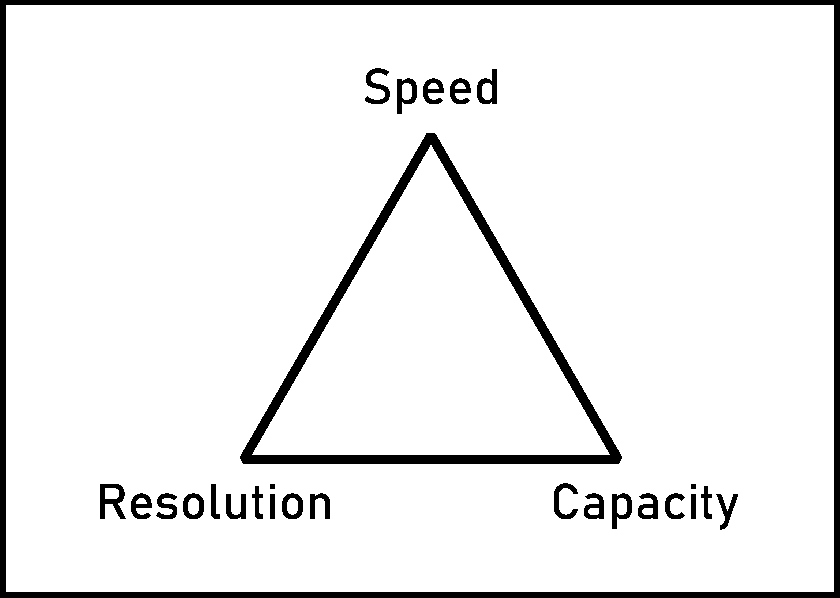
\includegraphics[width=\textwidth]{Figures/Triangle.pdf}
\decoRule

\caption[Schematic diagram of a the chromatograher's trilemma.]{The chromatographer's trilemma.}

\label{fig:trilemma}
\end{figure}

We avoided the trilemma by not bothering with optimizing column capacity. Sample
capacity in capillary GC is a function of film thickness and column diameter. We
decided to use the workhorse of GC, the \SI{0.25}{\milli\metre} internal
diameter column with a \SI{0.25}{\micro\metre} film thickness. The stationary
phase was a proprietary cross-linked polysiloxane polymer (Restek
Rxi\textregistered{}-5Sil MS), designed to mimic the behaviour of a
\SI{5}{\percent} diphenlyl/\SI{95}{\percent} dimethyl polysiloxane stationary
phase. With the phase ratio/column capacity fixed, the remaining trade-off is
between speed and resolution.

The experienced chromatographer will know that there is only one optimum flow
rate, the miniumum of the Van Deemter curve \(\hat{h}=\frac{B}{u}+C\), or under
high pressure drop conditions, the equivalent equation by Blumberg
\todo{autocite Blumberg} \(\hat{h}=\frac{B}{\bar{u}^2} + C_1\bar{u}^2 +
C_2\bar{u}\)

For a given column diameter and stationary phase, it is not possible to run a
faster chromatogram with higher resolution. Any attempt to increase the speed
will lead to lower resolution. If the flow is at an optimum, a shorter column
will yield a lower void time, but the number of plates will be lower so the
separation will not have the time to complete, resulting in decreased
resolution. If the column length is kept constant but the flow is increased, the
plate height will be lower, so the same length of column will have fewer plates, and hence
decreased resolution. 

For this reason, the official methods of separating the fatty acid methyl esters
(FAMEs) found in biodiesel require columns \SI{100}{\metre} long
\autocite{AOCS2017}, and run times of hours. This will generate just enough
resolution to separate the chemically very similary FAMEs

For any given column, the only way to make GC separations faster is to generate
excess resolution. Fewer theoretical plates will then be necessary to obtain an
optimal resolution. Excess resolution can be obtained by increasing the
selectivity $\alpha$, or by selective detection (\textit{e.g.} electron capture
detector). In practical terms this means using a column with a different
stationary phase or a different detector. 'A non-chromatographic way to generate
excess resolution is often termed `sample cleanup'. While not usually considered
part of chromatography, it is an additional separation step that removes
non-analyte compounds, so that only relevant compounds need to
separated form each other. 

In SFC$\times$GC excess resolution is generated in the \textsuperscript{1}D SFC
separation. By separating compounds by their group types first, the
\textsuperscript{2}D GC separation, in which separation is dominated by
volatility, needs a much lower resolution.

\begin{equation} 
N_{req} = 16R^2_s\left[\frac{1+k}{k}\right]^2\left[\frac{\alpha}{\alpha-1}\right]^2
\label{eqn:Nreq}
\end{equation}

The excess resolution can be traded for faster chromatography using 

\begin{itemize}
  \item Shorter columns
  \item Higher flow rates
  \item Temperature programming
  \item A combination of the above.
\end{itemize}

Fortunately the literature is quite clear . It
has been shown showed that superior resolution is obtained when shorter columns
are used rather than higher flow rates \autocite{Klee2002}. In her thesis Gail
Reed \autocite{Reed1999} compared shorter columns against faster flow, and
showed that shorter columns produce superior results over faster flow. Then she
concluded:
\begin{quotation}
Fast temperature programming should be used for fast
GC rather than a smaller internal diameter. Fast temperature programming has been
largely underutilized; however, new instrumentation will make it possible to more fully
exploit fast temperature programming rates. Fast temperature programming rates allow
for the use of short columns with normal i.d.s and film thicknesses which makes sample
capacity less of a problem for this mode of fast GC compared to other means of fast GC.
\end{quotation}

In line with this recommendation, the fast GC therefore used a short GC column
(\SI{1}{\metre} long) that used a correspondingly fast temperature program.

\section{Temperature programming}

Temperature programming is, of course, not necessary only for fast
chromatography, but has long been implemented to avoid the \textit{general
elution problem} \autocite{Skoog2007}. This problem can be summarized as
follows: in separations of complex mixtures, it becomes unlikely that one set
acceptable operating conditions (temperature, flow and stationary phase) will
give satisfactory (fast enough with acceptable resolution) separations for all
compounds of interest. As discussed above, there is only one optimum flow, and
it is impractical to change the stationary phase during a run, so the only
parameter to change is the temperature.

The technology for temperature programming in GC is well developed, and every
column stationary phase has specified temperature limits for isothermal and
programmed use.

\section{Temperature ramp rates}

When early experimenters realized the importance of temperature control in GC,
they used oil baths, but quickly realized that leaks could allow oil into the
column. Oil that entered the column would then contaminate the stationary phase,
rendering it useless. Therefore, in the modern, conventional gas chromatograph
the column is heated in an air bath with very precise temperature control. These
are baths are capable of temperature ramps of perhaps a hundred Celsius degrees
per minute. 

Blumberg and Klee \autocite{Blumberg2000} recommend that a good initial
temperature ramp rate is 10 C\textdegree{} per void time ($t_m$). For long
columns the void times are long, and the ramp rates can be low. As illustration,
Figure \ref{fig:RampRate7890B} shows the temperature ramp rates of a
state-of-the-art chromatograph. By contrast, for short, narrow-bore columns, the
ramp rate needs to be thousands of celsius degrees per minute.

\begin{figure}
	\centering
	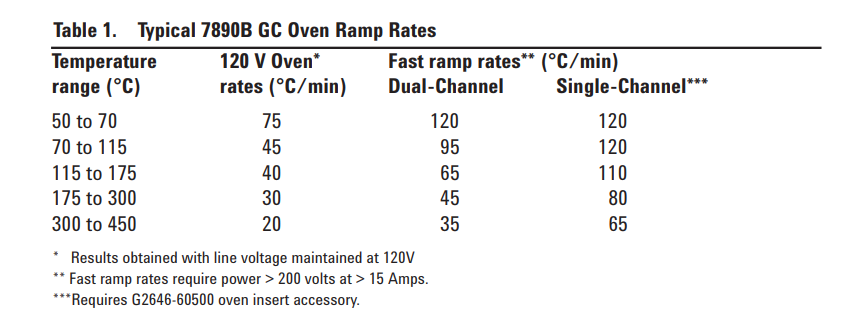
\includegraphics[width=0.8\textwidth,natwidth=4.17in,natheight=3.32in]{Figures/7890B.png}
	\decoRule
\caption[A temperature-rate table from the Agilent7890B data sheet]{The temperature-rate table from the Agilent 7890B chromatograph data sheet\autocite{7890B}. }
\label{fig:RampRate7890B}
\end{figure}


The low ramp rate of conventional air baths are cause by three factors:

\begin{itemize}
	\item The low heat capacity of air
	\item The poor thermal conductivity of air
	\item The mass of the oven that needs to be heated. 
\end{itemize}

There is very little that can be done about these matters. In theory it would be
possible to switch oven gas to hydrogen for higher thermal conductivity, and
construct a low-mass oven using, say, advanced resins for construction, but this
would probably involve significant safety and cost issues. 

\subsection{Resistive heating}

Fortunately the heating rate problem has a technologically simple solution,
\textit{resistive heating}. When a constant electric field is applied to a metal, the
free electrons in the metal will be accelerated by the electric field. But the
electrons are within the crystal lattice of the metal, and the mean free path is
very short. The electrons will therefore collide with atoms in the crystal
lattice, scattering inelastically. The energy lost in the inelastic collisions
will increase the vibrating frequency of atoms, and this energy will appear as
heat. The number of electrons and their average (drift) speed will determine the
current ($I$), and the electric field is best described by the applied voltage
($V$). The current $I$ is proportional to the applied voltage, and the ratio
$\frac{V}{I}$ defines the proportionality constant $R$, called the resistance.
The total power dissipated to heat ($P$) is given by the equation $P=IV$ or,
equivalently, $P=I^2R$ or $P=\frac{R}{V^2}$.

(Alternative methods of heating by electromagnetic fields are \textit{inductive
heating} and \textit{dielectric heating})

The rate at which the piece of metal heats up depends on the power dissipated,
the mass of the metal, and its heat capacity. Applying a voltage $V$ to a metal
element in close proximity to the column will heat the metal, and therefore the
column in contact with it. If the volume of the metal is small enough, and the
current high enough, the temperature of the metal element will increase, and
with it the temperature of the column, which can then be changed at any
desirable rate.

This technology has been reviewed \todo{autocite resistive heating reviews}, and
a few technologies have emerged.

\begin{itemize}
  \item Metallic columns \todo{Check review for kinds}
  \item Columns coated with metal layers
  \item Collinear heating
  \item Coaxial heating
\end{itemize}

For reasons that will become clear, we decided on using coaxial heating. 

\begin{figure}[htbp]
	\centering
	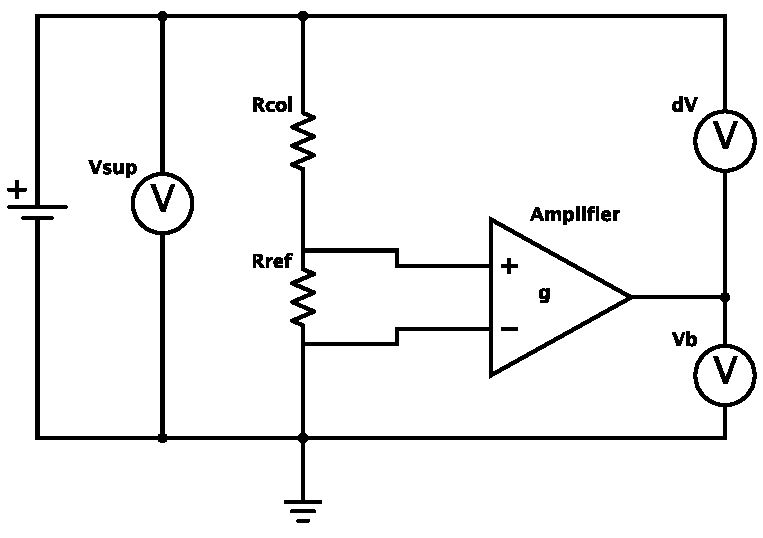
\includegraphics[width=0.8\textwidth,natwidth=4.17in,natheight=3.32in]{Figures/Column-Heater.pdf}
	\rule{35em}{0.5pt}
	\caption[Coaxial heater resistance heater]{Electric circuit diagram of the coaxial heater.}
	\label{fig:HeaterDiagram}
\end{figure}

The circuit is supplied by a voltage $V_{sup}$, in general an unknown value.
$V_{col}$ and $V_{ref}$ represents the voltage drop over the respective
resistors.

Because the current $I$ through the circuit is the same for both $R_{col}$ and
$R_{ref}$, it is true that $\frac{R_{col}}{V_{col}}=\frac{R_{ref}}{V_{ref}}$,
and therefore \begin{equation}R_{col} = R_{ref}\frac{V_{col}}{V_{ref}}
\end{equation}

The voltage drop across $R_{ref}$ is small, and therefore it is amplified by the
amplifier with gain $g$, so that $V_b = gV_{ref}$. $V_b$ is measured, as is
$dV$, the potential difference between the supply and the amplifier output.

$V_{sup} = V_{col} + V_{ref}$ 

$V_{sup}=dV + V_b$

$V_{col} + V_{ref} = dV + V_b$

$V_{col} + V_{ref} = dV + gV_{ref}$

$V_{col} = dV + gV_{ref} - V_{ref} $

$V_{col} = dV + V_{ref}(g - 1)$

$\frac{\displaystyle V_{col}}{\displaystyle gV_{ref}} = dV/gV_{ref} + V_{ref}(g-1)/gV_{ref}$

$\frac{\displaystyle V_{col}}{\displaystyle V_{ref}} = gdV/gV_{ref} + gV_{ref}(g-1)/gV_{ref}$

$\frac{\displaystyle V_{col}}{\displaystyle V_{ref}} = gdV/V_b + (g-1)$

This proves that $\frac{\displaystyle V_{col}}{\displaystyle V_{ref}}$ is a
linear function of $dV/V_b$. A quick check for correctness of the expression:
for a unity-gain amplifier $g = 1$, and $\frac{\displaystyle
V_{col}}{\displaystyle V_{ref}} = dV/V_b$.


\subsection{Assumptions}

The assumption is that the temperature is a function of the resistance of the
column, or $T = f(R_{col})$. Because $R_{col}=m(^{dV}/_{V_b}) + c$, we can say
that $T = f'(^{dV}/_{V_b})$. Through a calibration procedure $f'$ can be
approximated by a polynomial.

\subsection{Cold spots}

For fastest temperature programming the heating element should be as light as
possible, and carry the largest necessary current. In practice, the current
doing the heating must be carried to the coaxial heater using a conductor. To
prevent the conductor from heating up it must have a low resistance, and this
low resistance is achieved by making the conductor as 'thick' or as 'heavy' as
necessary, meaning that it should be constructed of a material with a high mass per unit
length.

Good electrical metallic conductors are invariably also good thermal
conductors, and therefore the area around the junction of the feed conductor to
the coaxial heater will always have a lower temperature than the nominal
temperature of the heater. In capillary GC this is undesirable: a cold spot in a
column can wreak havoc with retention times and peak shapes. 

The electrical connection between the feed conductor and the coaxial heater was
therefore designed in the form of an externally heated block. This block was
kept at a higher temperature than the highest expected temperature of the
chromatographic temperature program. This prevented the formation of cold spots
in the coaxial heater, which might lead to cold spots in the column.
 

\section{Sample injection/modulation}

In the SFC$\times$GC system described here. 

\todo{Two-stage modulator}

\subsection{Restrictor}


\subsection{Cold column}

\section{Column}

\subsection{Column heating}

\subsection{Heating control and temperature programming}

\subsection{Temperature uniformity}
\label{sec:Uniformity}

\subsection{Temperature calibration}

The problems of measuring a temperature inside a tube with a bore of \SI{0.8}{\milli\metre} is not trivial.

The following technologies exists to measure temperatures:
\begin{itemize}
	\item Liquid-in-glass thermometers
	\item Sealed liquid or gas sensing instruments and bimetallic sensors.
	\item Electrical resistance temperature measurement using metallic sensors
	\item Thermistors and semiconductors
	\item Thermoelectric temperature measurement
	\item Disappearing filament optical pyrometer
	\item Photoelectrical optical pyrometers
	\item Total radiation pyrometers.
\end{itemize}

Liquid-in-glass thermometry would not be applicable because of the size of the
devices, and because they don't give a desirable electrical signal. 

In recent years the technology for measuring temperature by radiant energy
methods have improved markedly and has become affordable, in the form of thermal
cameras. However, at lower temperatures the accuracy of the recorded temperature
depends heavily on the emissivity of the measured material. Thermal imaging will
also only measure the outside wall surface temperature of the heater, and not
the temperature of the inside of the coaxial heater. So, while thermal imaging
settled questions about heater uniformity (Section \ref{sec:Uniformity}), it was
not considered ready to serve as a calibration standard. 

This leaves us with resistance temperature measurement with metallic
sensors, thermistors and semiconductors, and thermoelectric.

Thermistor and semiconductor devices could, in principle be made small enough
for the job, but affordable packages are too large. Besides that, the operating
temperature range is a bit extreme for semiconductors that generally have an
upper temperature limit of about 200  \si{\celsius}. \todo{Mil-spec temperature range}

Electrical resistance measurement using metallic sensors are quite feasible, if
a sensing element of the right dimensions are available. These are not easy to
find. Additionally, because long thin wires would be needed to connect the
sensing element to the electronics, correction for those conductors would have to be made. 

Thermoelectric temperature measurement then remains. This uses the effect that a
circuit of two dissimilar metals will generate a voltage when there is a
temperature gradient along the conductors. The voltage generated is a function
of the temperature difference between the junctions of the two metals. Such a
pair of dissimilar conductors used to generate a voltage is known as a
\textit{thermocouple}. Thermocouples are widely used in industry for measuring
temperatures, and the technology is well established. Thermocouple wire can be
purchased in varying gauges, down to \SI{25}{\micro\metre} in diameter, and the signal
processing for thermocouple signals have been standardized.

McGee \autocite{Mcgee1988} states that thermocouple junctions can be made by
welding, crimping, soft soldering, hard soldering, bolting, or simply twisting
the wires together.

Because of the temperature range expected to be measured ({-}50 \si{\celsius} to
400 \si{\celsius}) the option of soft soldering does not apply, because soft
solders have a melting points around \SI{200}{\celsius}. The
possibility of corrosion and mechanical vibration suggest that twisting the wires together is
will not form a reliable joint, and of course there are no sub-millimetre bolts on the market.

This leaves welding, crimping and hard soldering. The option of crimping was not
explored, chiefly because we have no knowledge of technology or devices that can
crimp hair-fine wire. Our knowledge of crimping suggest that shows another
problem: the final crimped connection has a diameter many times the diameter of
the wire. This precludes the application of crimping in this context.

Hard soldering is usually done with high-temperature flames, and on contact the
flames will rapidly burn the fine wires. The temperatures required for hard
soldering is still lower than the melting point of the wires, so that hard
soldering is not excluded, but we did not have the knowledge or the technology
to solve the associated problems.

Welding was found to be an accessible technology for forming small, reliable
joints in fine fine thermocouple wire.

\subsection{Thermocouple Welding}

\begin{figure}
	\centering
	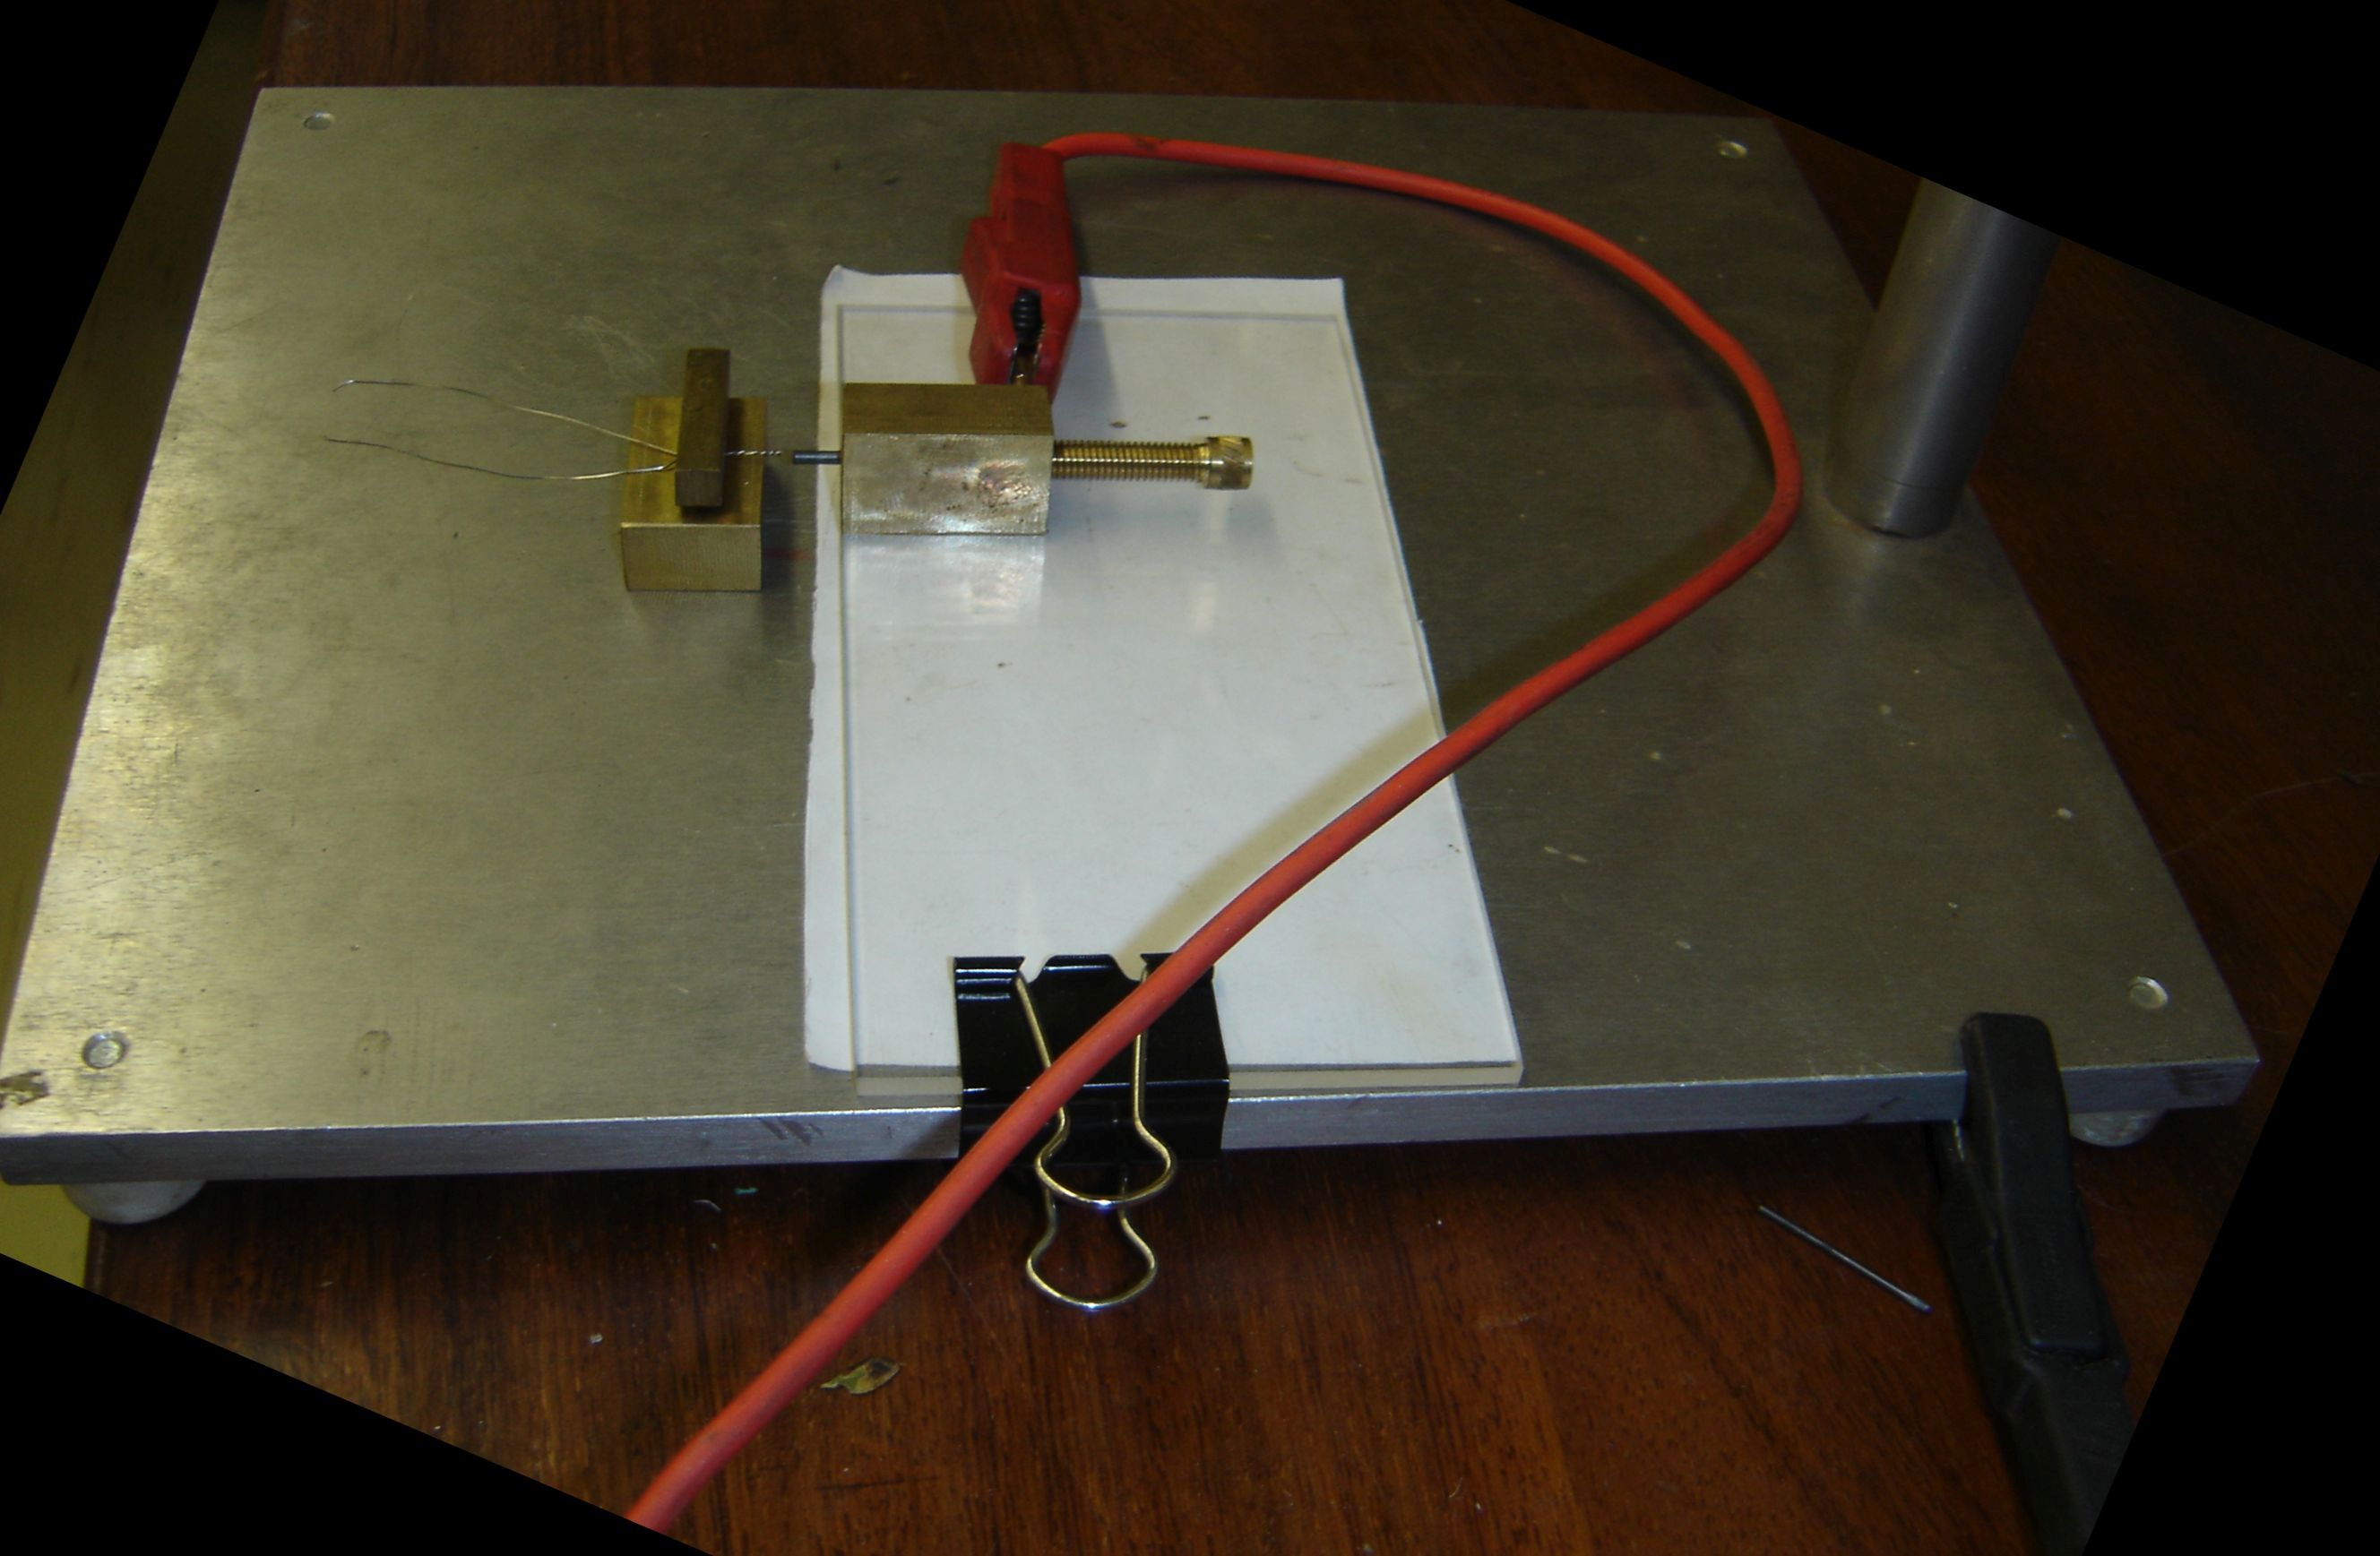
\includegraphics[width=0.8\textwidth,natwidth=4.17in,natheight=3.32in]{Figures/Welder2.jpg}
	\decoRule

\caption[Fine-wire welder]{A view of the fine-wire thermocouple welder. The wire
shown is much thicker than that actually used. It is shown clamped between the
clamping bar and the clamping weight. A thin sheet of Perspex serves to isolate
the positive electrode from the negative base. The carbon electrode can be
advanced towards the thermocouple twist using the screw. The black clamp at the
bottom right-hand corner attached to the base plate and the red clamp attached
to the screw housing provide a potential difference of approximately 20 V
between the carbon electrode and the thermocouple.}


\label{fig:FireWireWelder}
\end{figure}



\begin{figure}
	\centering
	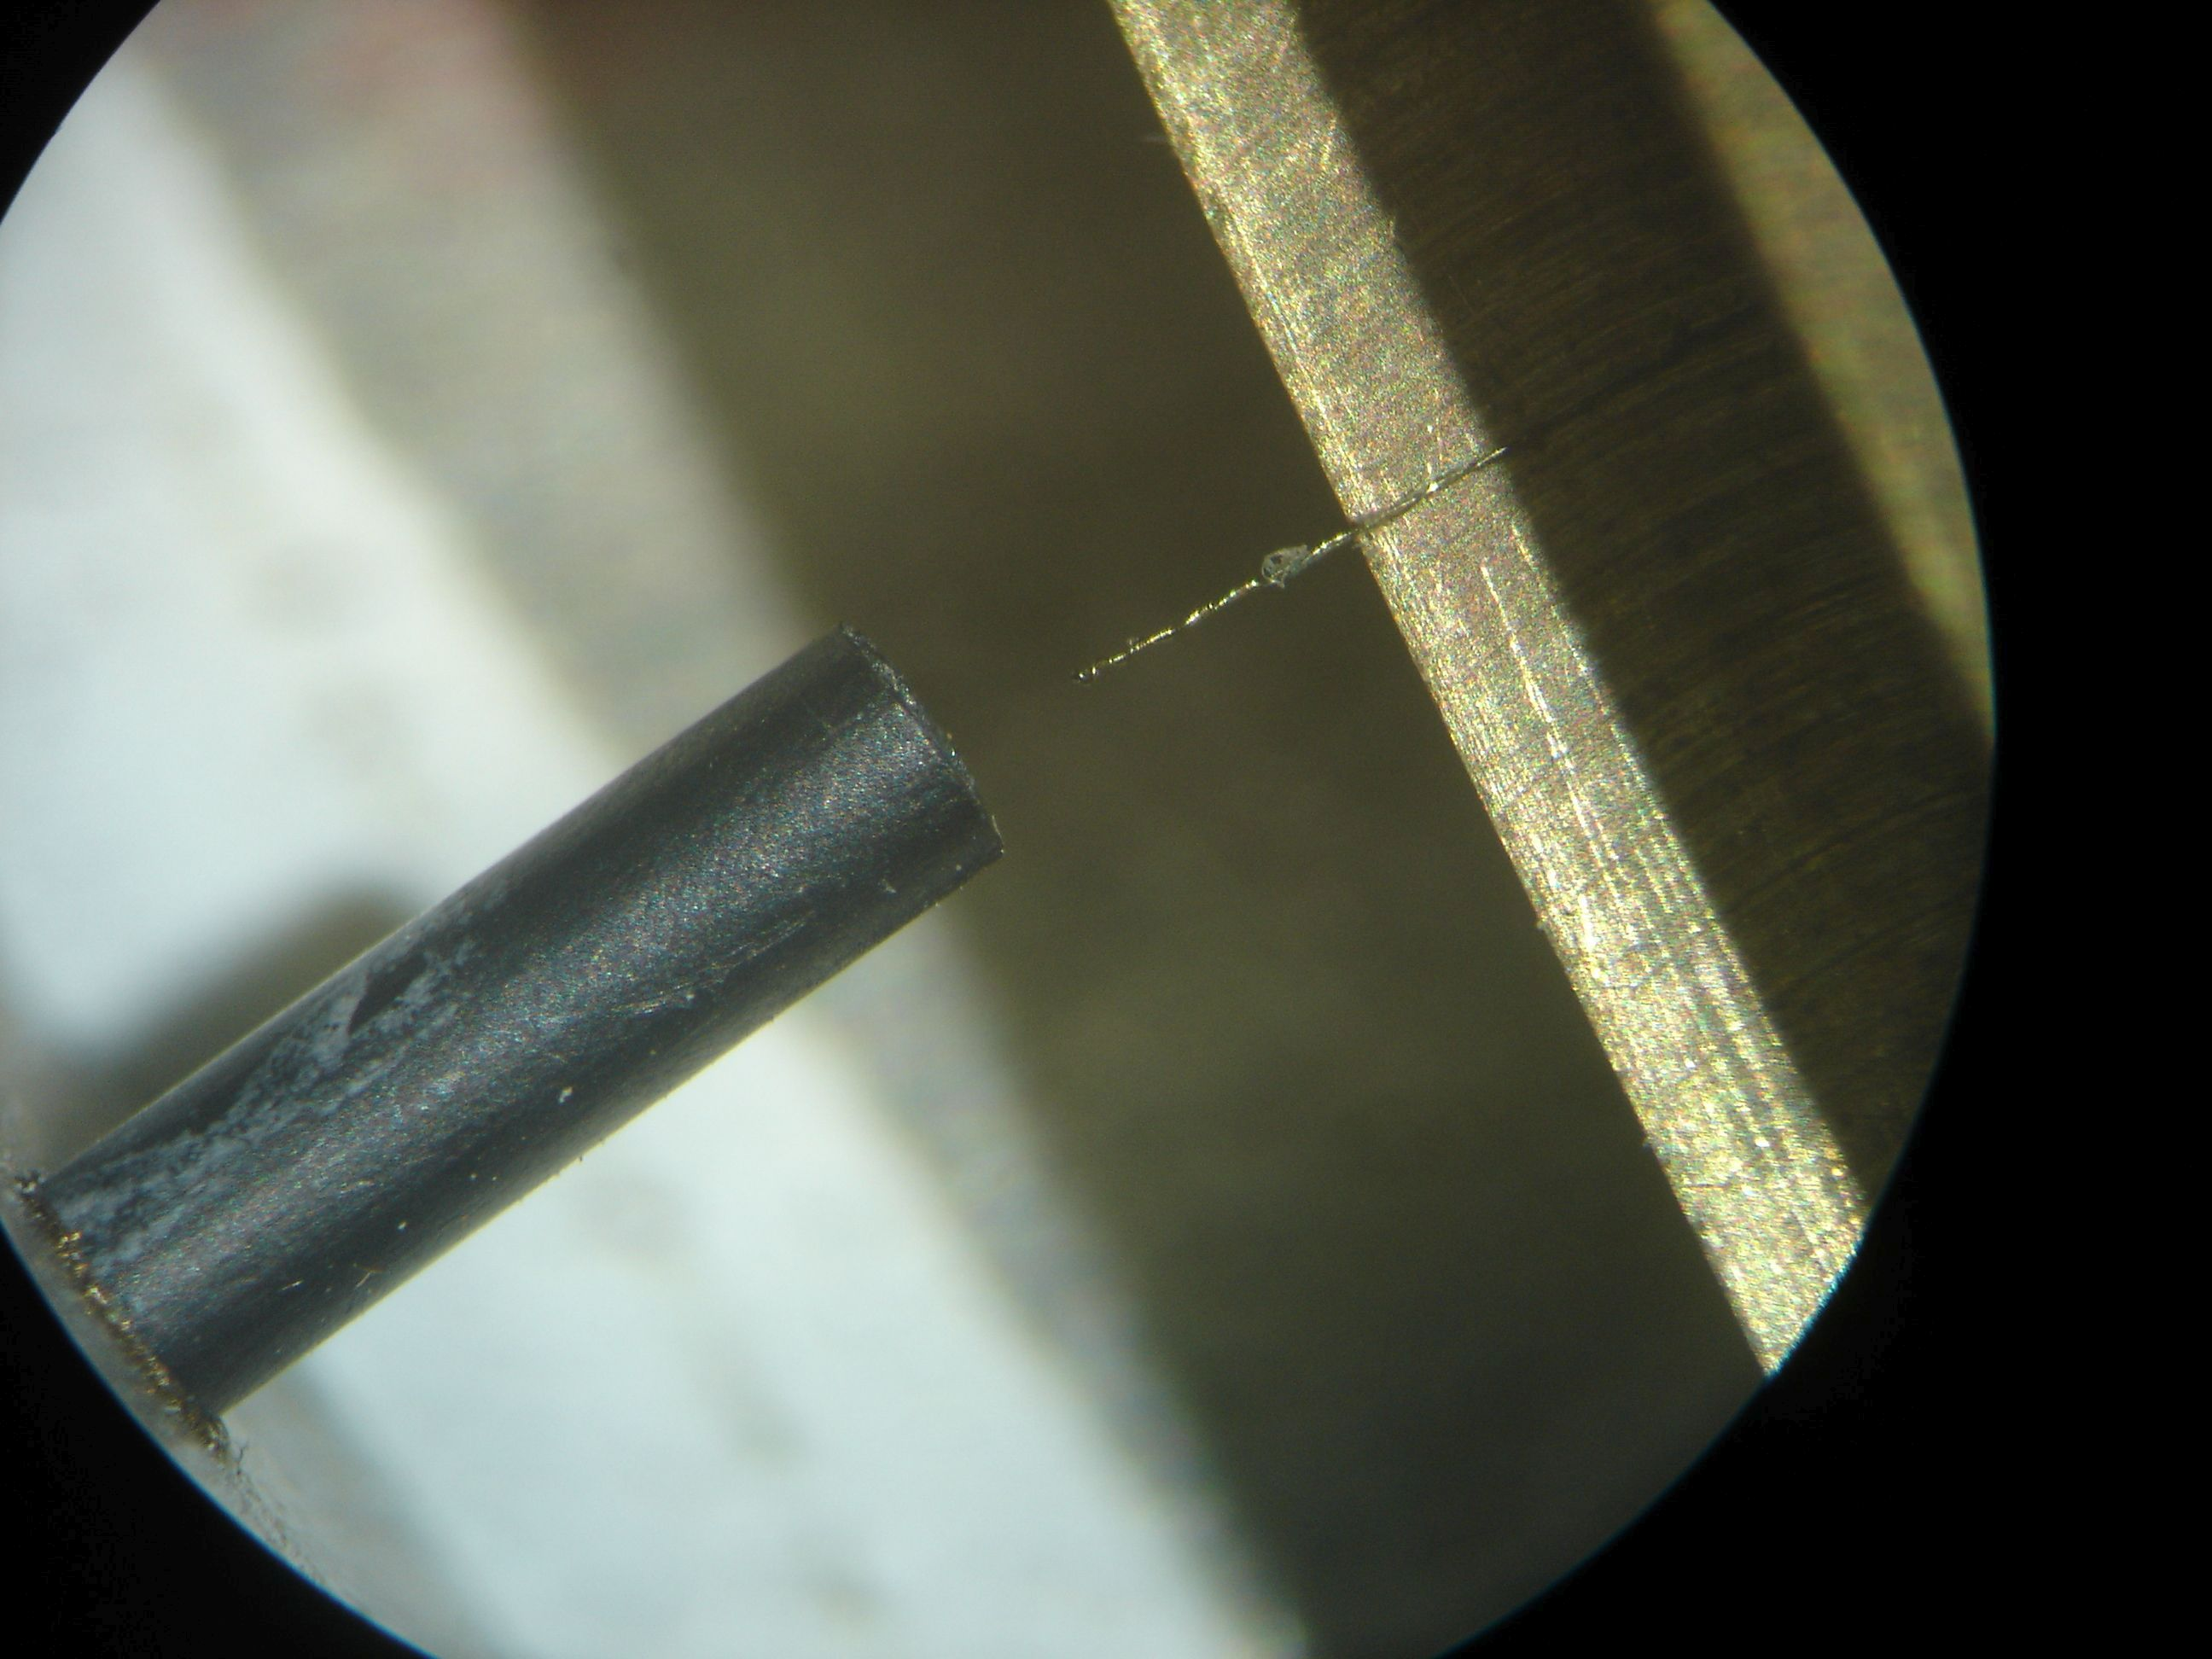
\includegraphics[width=0.8\textwidth,natwidth=4.17in,natheight=3.32in]{./Figures/WelderMicro.jpg}
	\decoRule
	
\caption[A microphoto of a thermocouple twist ready to be welded.]{A microphoto
of a twisted wire ready to be welded. The black carbon electrode is 2mm in
diameter.}
	
	\label{fig:TheFigureLabel}
\end{figure}

\subsection{Termocouple probe construction}

\begin{figure}
	\centering
	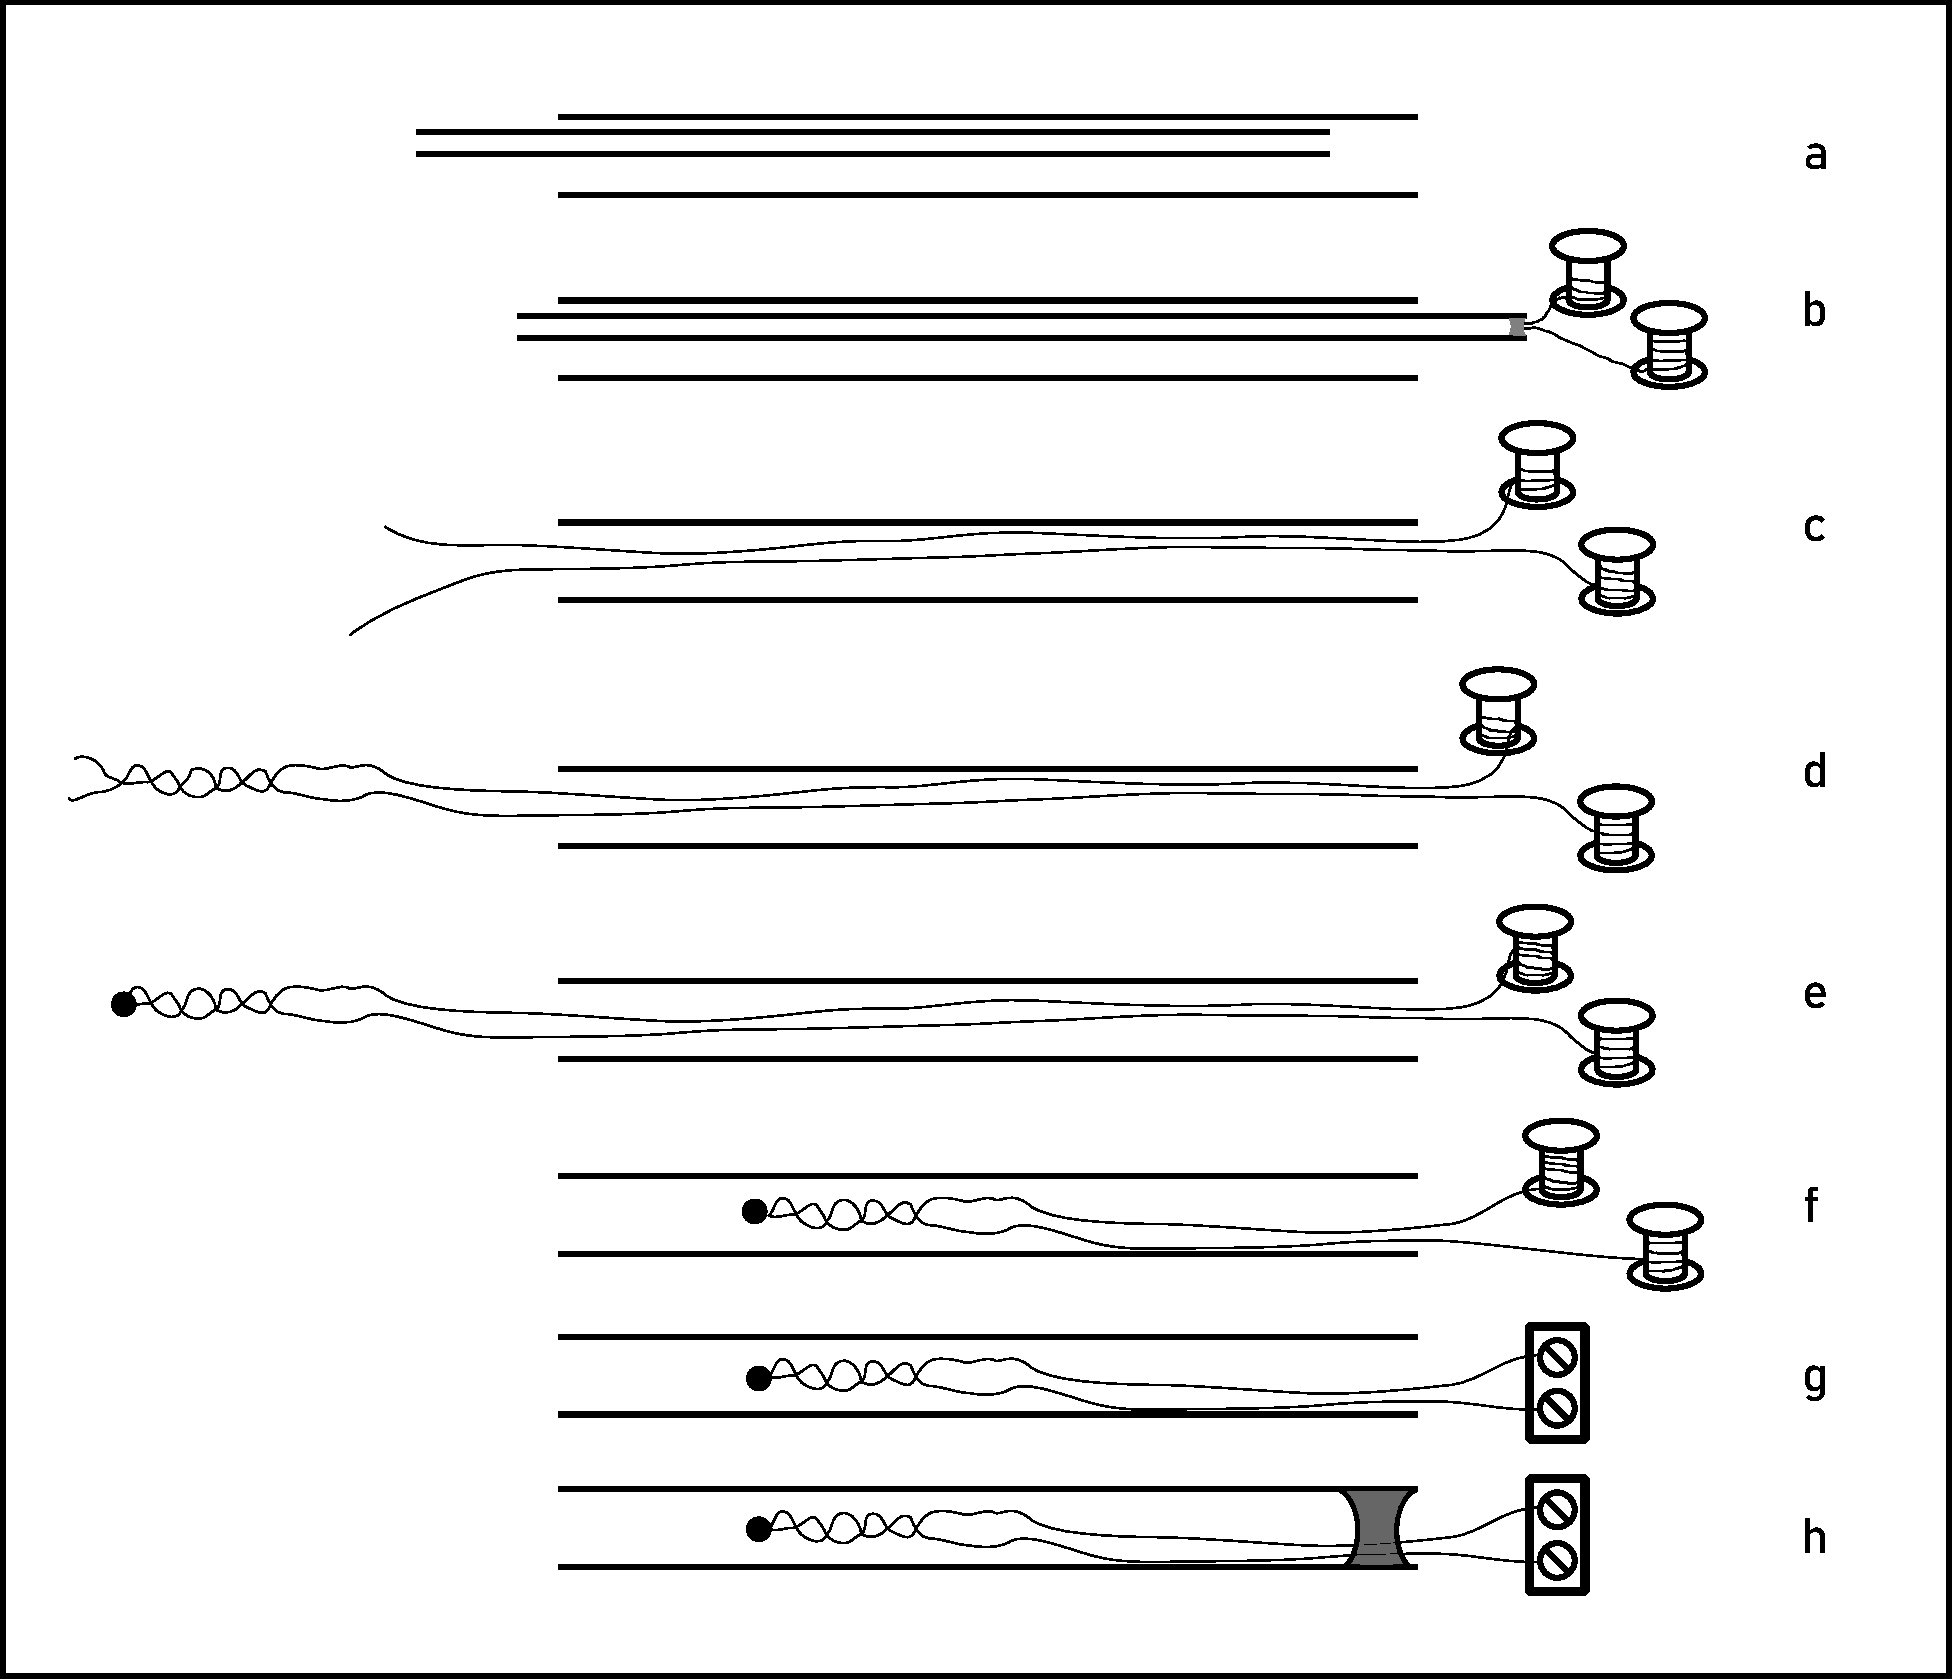
\includegraphics[width=0.8\textwidth]{./Figures/FineWireThermocouple.pdf}
	\decoRule
	
\caption[A cartoon explaining how to construct a long, thin thermocouple
probe.]{(a) A thin capillary is threaded inside a thicker one (b) The ends of a
pair of thermocouple wires are fitted inside the end of the thin capillary. (c)
The wires are pulled through the thick capillary using the thin capillary. (d)
The ends of the wires are twisted together, creating a mutual mechanical anchor.
(e) The ends of the wires are welded together. (f) The wires are pulled back
into the thick capillary, locating the junction at the desired position in the
capillary. (g) The wires are trimmed and connected to a terminal block. (h) A
drop of cyanoacrylate adhesive is used to anchor the wires permanently in the
capillary. }
	
	\label{fig:FineWireThermocouple}
\end{figure}

\subsection{Column cooling}

\todo{Drawing of heat exchanger}

\subsection{Column mounting}


The T-piece blocks described elsewhere\todo{refer to section/page describing
T-piece block} acted as a mounting point for the coaxial heater. The block is
quite heavy, and has to transmit the forces of the coolant tube and the
electrical connections. The column runs from the heated inlet/detector to the
heated T-piece block, and in between it should not be exposed to any
low-temperature cold spots, therefore the gap between the T-piece block and the
inlet/detector should be quite small. But the gap cannot be zero, because
electrical isolation needs to be maintained. A mechanically stiff and accurate
mounting was needed for the T-piece blocks, to allow the precise but
adjustable alignment of the T-piece blocks and the inlet/detector.

Through a few iterations a parallel-rail design was developed. These rails were
held in place in the Varian 3300 oven by friction, so that they could be
adjusted and removed as necessary, yet was stiff enough to transfer the
necessary forces without deflecting. Figure \ref{fig:RailsDrawing} shows a
technical drawing of the rails as designed. 

\begin{todo}

Make sure all the information in this paragraph is captured: The pointed ends of
the rails pressed against a solid aluminium plate used as the floor of the oven,
and the top, adjustable points pressed against pressure plates which pressed
against the roof of the oven. This formed a complete, rigid structure that could
be installed in the Varian 3300 GC oven without making any modifications to the
oven. The column could then be installed in the oven by putting the T-piece
mounting blocks on the cars.

\end{todo}

\begin{figure}
	\centering
	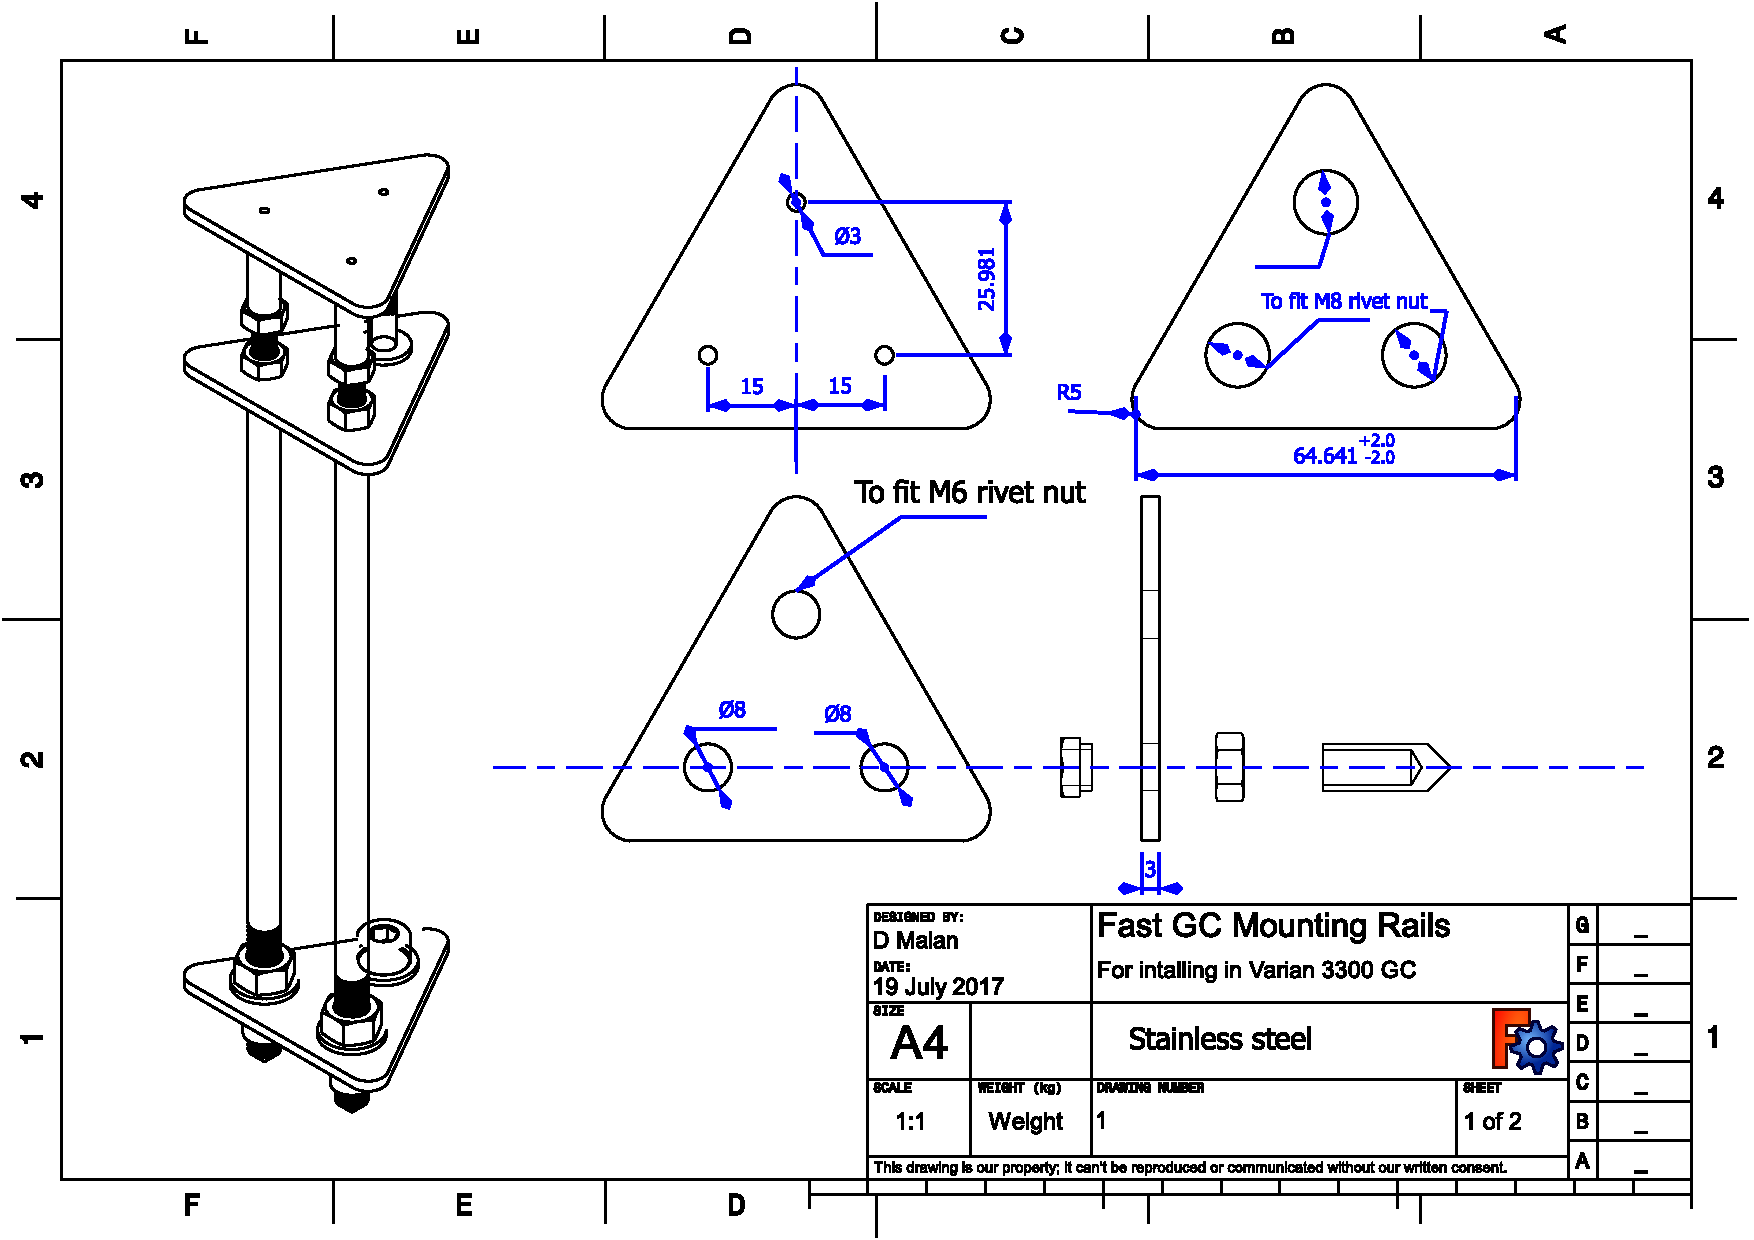
\includegraphics[angle=90, origin=c, scale=0.75]{Figures/RailsDrawing.pdf}
	\decoRule	
\caption[Technical drawing of coaxial heater mounting rails]{\label{fig:RailsDrawing}A technical drawing of the rails carrying the T-piece mounting block.} 
	
\end{figure}

The T-piece blocks was the electrical connection for the resistive coaxial heater,
which meant they needed to be electrically isolated, but they were also heated
which meant that the insulation had to be heat resistant. A commercial available
material that met these requirements was found in the form of \textit{silicon
mica}, a composite material of mica and a silicone resin. This material has a
continuous operating temperature of at least \SI{500}{\celsius}, making it
ideally suited to GC applications. The silicon mica is also easy to machine, so
that it could he shaped to the necessary specifications.

The T-piece blocks were mounted on a pair of cars riding on the round-bar rails.
The cars comprised a sandwich design of layers of stainless steel and silicon
mica around a pair of brass bushes. Once assembled, the cars offered a set of
studs on to which the user could slide and bolt down the T-piece blocks. The
position of the cars were determined by a locking collar on one of the rails.
Figure \ref{fig:CarsDrawing1} shows technical drawings of the cars that explains
the design.

\begin{figure}
	\centering
	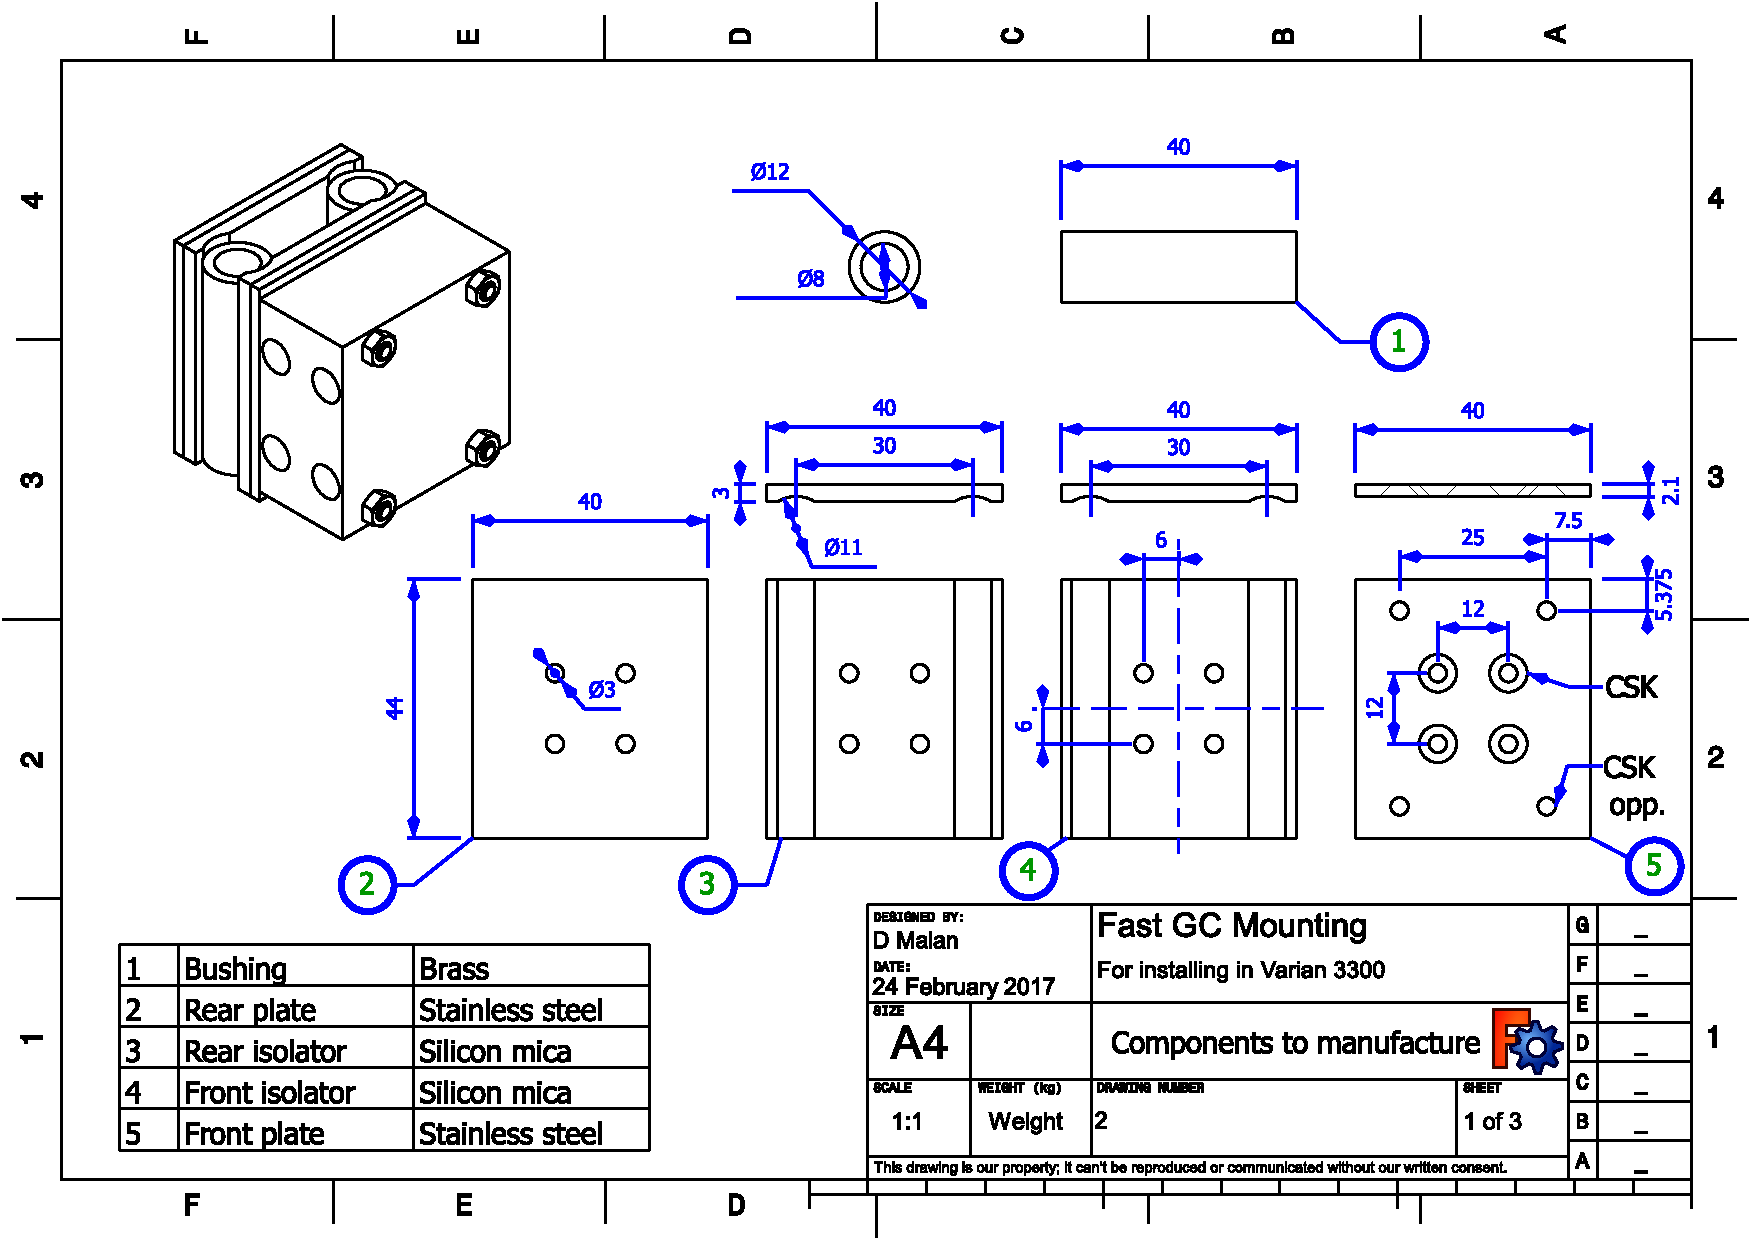
\includegraphics[angle=90, origin=c, scale=0.75]{Figures/CarDrawing1.pdf}
	\decoRule	
\caption[Technical drawing of coaxial heater mounting.]{A technical drawing of the T-piece block mounting.} 
	\label{fig:CarsDrawing1}
\end{figure}

\begin{figure}
	\centering
	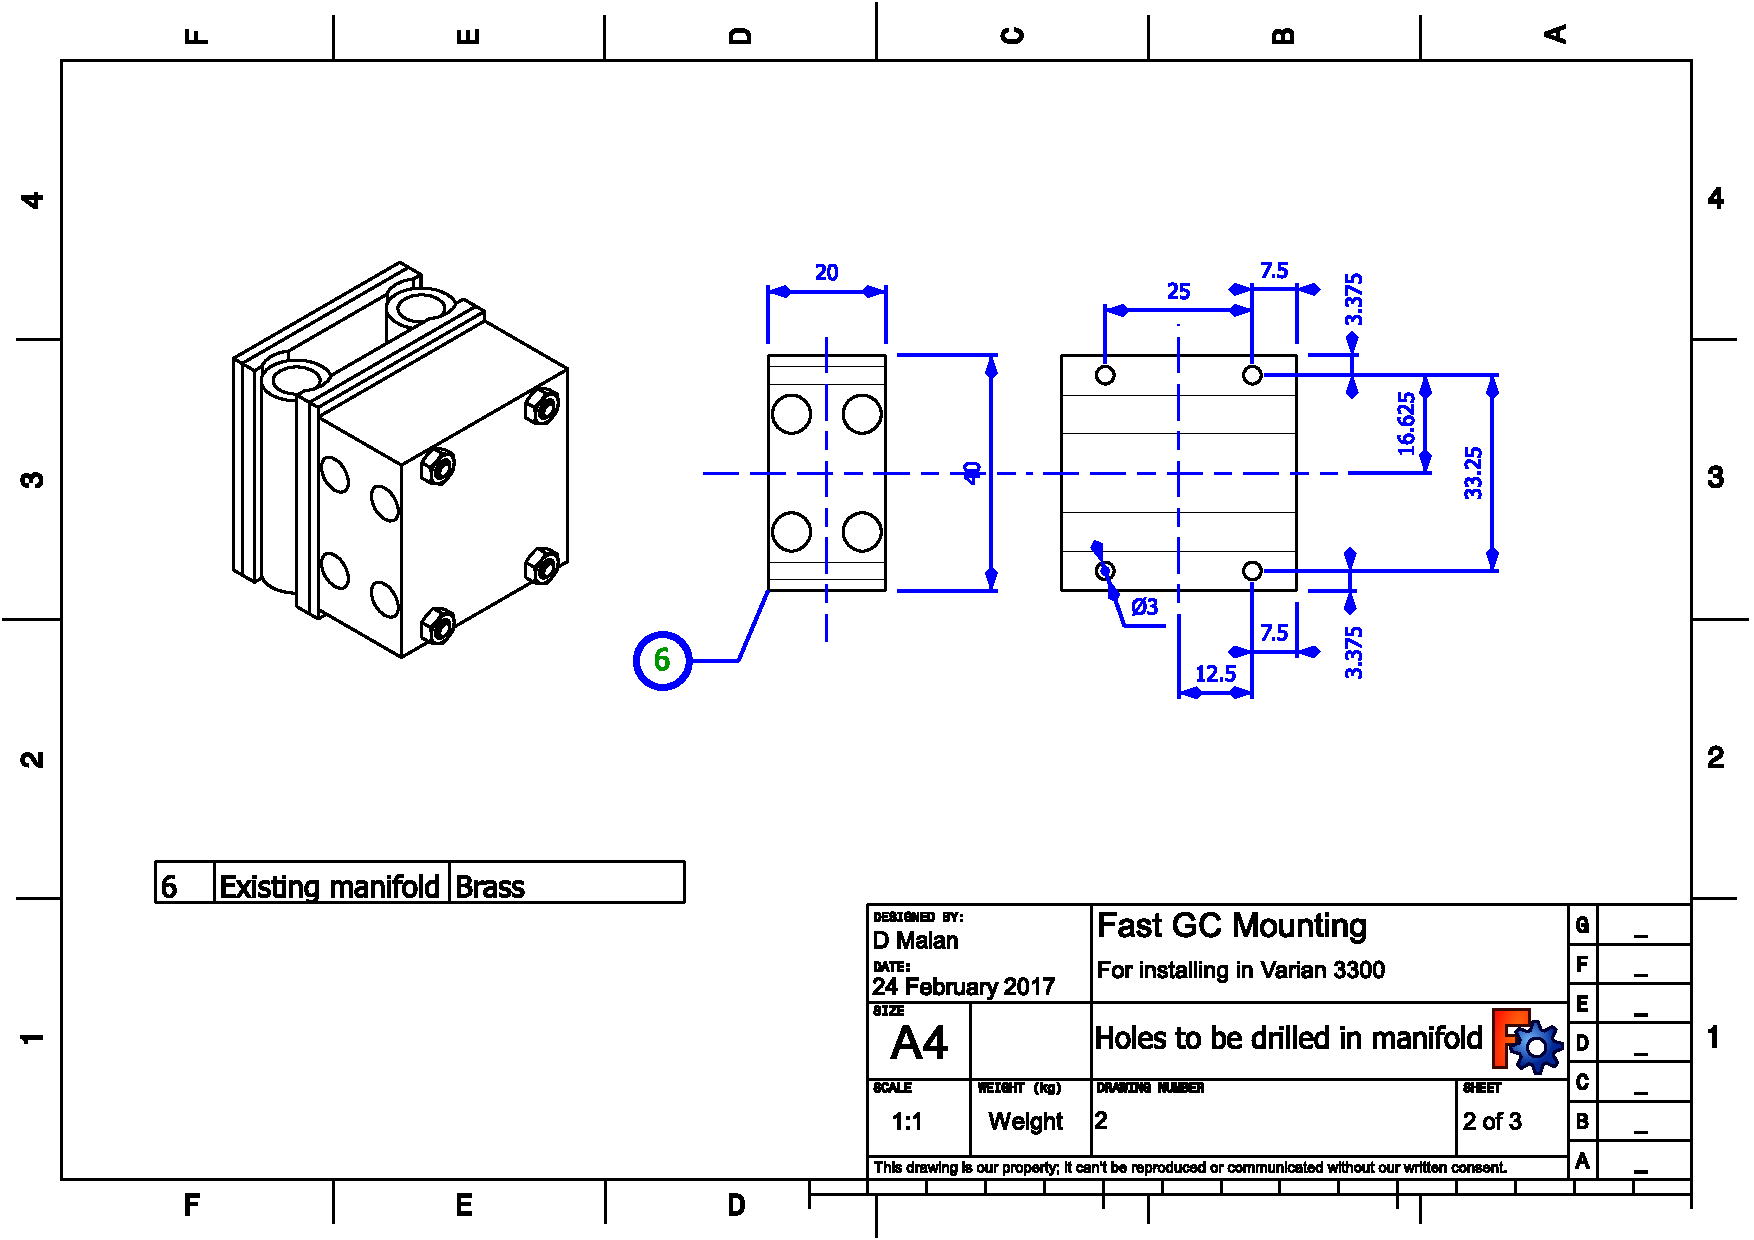
\includegraphics[angle=90, origin=c, scale=0.75]{Figures/CarDrawing2.pdf}
	\decoRule	
\caption[Technical drawing of coaxial heater mounting.]{A technical drawing of the T-piece block mounting.} 
	\label{fig:CarsDrawing2}
\end{figure}

\begin{figure}
	\centering
	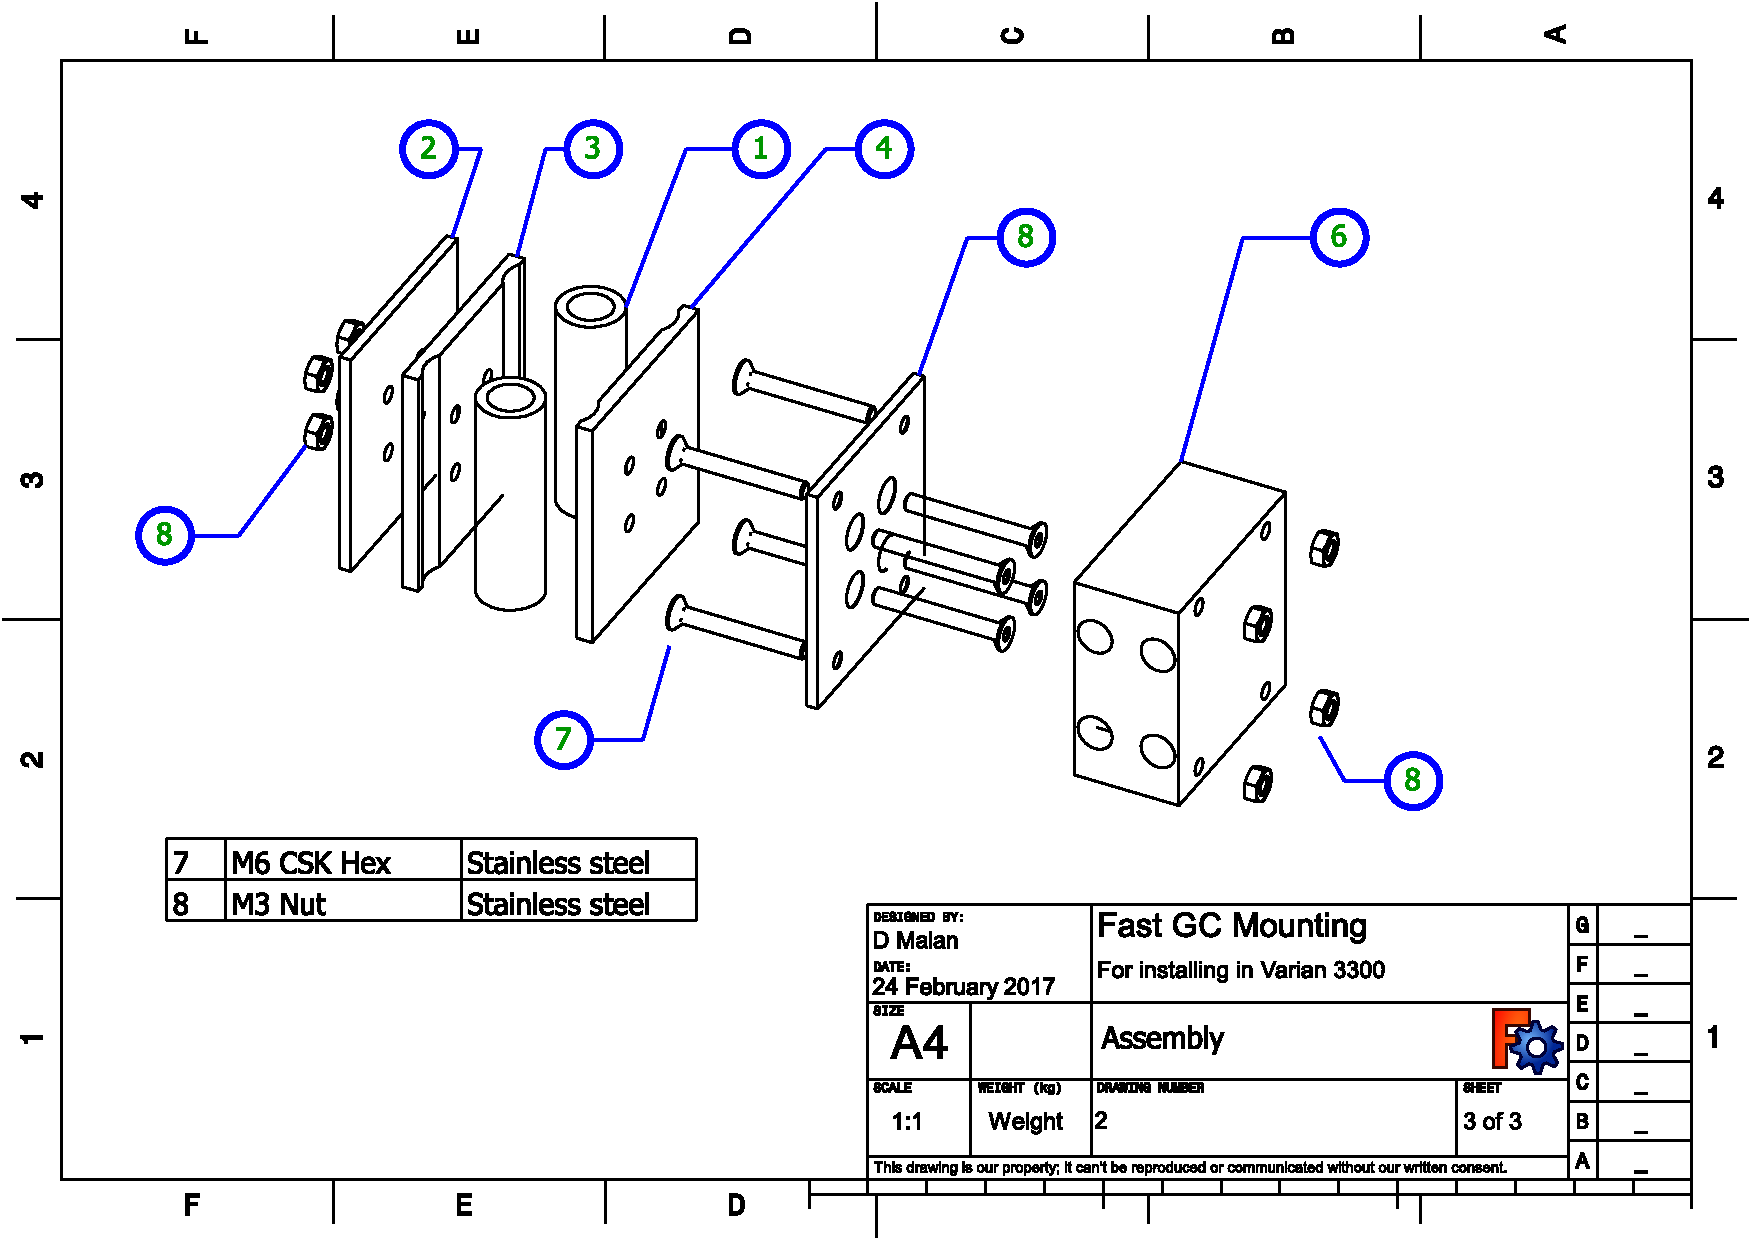
\includegraphics[angle=90, origin=c, scale=0.75]{Figures/CarDrawing3.pdf}
	\decoRule	
\caption[Technical drawing of coaxial heater mounting.]{A technical drawing of the T-piece block mounting.} 
	\label{fig:CarsDrawing3}
\end{figure}

\todo{Use Figure environment instead of includepdf. \\
Use caption package to suppress labelling of continued figures \\. 
https://tex.stackexchange.com/questions/64231/how-can-i-create-a-continued-figure-caption}



\section{Detector}

The detector used in this fast GC was an unmodified Varian\texttrademark{} 3300
Flame Ionization Detector. The detector bias voltage was supplied by the
original electronics, but a stand-alone high-speed electrometer (V.G. Micromass
Ltd, Model M406-H) captured the signal, which was then conditioned by a
bench-top amplifier (V.G. Micromass Ltd, Model M406) before it was sent to the
computer. This electrometer and amplifier were fast enough to detect and amplify the signals generated by the fast GC. 

\section{Data capture}

In GC$\times$GC, 2D data is recorded as a continuous FID output stream, as if it
is a 1D GC chromatogram, and later converted into a 2D chromatogram, using
knowledge of the modulation period.

For two reasons we could not use this approach. Firstly, in our instrument the
first (SFC) dimension runs in a stop-flow mode making continuous data recording
inappropriate. Secondly, the duration of the cooling cycle varies, which would
introduce unacceptable variation in \textsuperscript{2}D retention times.

We therefore constructed 2D chromatograms by starting to record data each time
the GC fast temperature program started, noting the GC start time as the elution
time of the first (SFC) dimension.

\section{Data visualization}
For data visualization we used the technical computing system Mathematica
11.3\texttrademark{} (Wolfram).  First the collected data was converted to a
list of three-element lists, with $^1$D retention time, $^2$D retention time,
and detector signal as the elements of the inner lists. The Mathematica
functions \texttt{List3DPlot[]} and \texttt{ContourPlot[]} could then be used to
plot 3D chromatograms or contour plots respectively.


\todos

